% !TEX TS-program = XeLaTeX
% use the following command:
% all document files must be coded in UTF-8
\documentclass[spanish]{textolivre}
% build HTML with: make4ht -e build.lua -c textolivre.cfg -x -u article "fn-in,svg,pic-align"

\journalname{Texto Livre}
\thevolume{15}
%\thenumber{1} % old template
\theyear{2022}
\receiveddate{\DTMdisplaydate{2022}{4}{7}{-1}} % YYYY MM DD
\accepteddate{\DTMdisplaydate{2022}{6}{4}{-1}}
\publisheddate{\DTMdisplaydate{2022}{7}{5}{-1}}
\corrauthor{Ana Manzano-León}
\articledoi{10.35699/1983-3652.2022.39171}
%\articleid{NNNN} % if the article ID is not the last 5 numbers of its DOI, provide it using \articleid{} commmand 
% list of available sesscions in the journal: articles, dossier, reports, essays, reviews, interviews, editorial
\articlesessionname{reports}
\runningauthor{Manzano-León et al.} 
%\editorname{Leonardo Araújo} % old template
\sectioneditorname{Daniervelin Pereira}
\layouteditorname{Carolina Garcia}

\title{Aprendizaje-Servicio lúdico en la formación inicial docente: un estudio cualitativo}
\othertitle{Aprendizagem-Serviço lúdica na formação inicial de professores: um estudo qualitativo}
\othertitle{Playful Service-Learning in initial teacher training: a qualitative study}
% if there is a third language title, add here:
%\othertitle{Artikelvorlage zur Einreichung beim Texto Livre Journal}

\author[1]{Ana Manzano-León  \orcid{0000-0001-6966-0355} \thanks{Email: \href{mailto:aml570@ual.es}{aml570@ual.es}}}
\author[2]{Ana María Ortiz-Colón  \orcid{0000-0003-0440-6107} \thanks{Email: \href{mailto:aortiz@ujaen.es}{aortiz@ujaen.es }}}
\author[2]{Javier Rodríguez-Moreno \orcid{0000-0002-5890-3654}
\thanks{Email: \href{mailto:jrmoreno@ujaen.es}{jrmoreno@ujaen.es}}}
\author[1]{José Manuel Aguilar-Parra \orcid{0000-0002-6703-0680} \thanks{Email: \href{mailto:jmaguilar@ual.es}{jmaguilar@ual.es}}}
\affil[1]{Universidad de Almería, Departamento de Psicología, Almería, España.}
\affil[2]{Universidad de Jaén, Departamento de Pedagogía, Jaén, España.}

\addbibresource{article.bib}
% use biber instead of bibtex
% $ biber article

% used to create dummy text for the template file
\definecolor{dark-gray}{gray}{0.35} % color used to display dummy texts
\usepackage{lipsum}
\SetLipsumParListSurrounders{\colorlet{oldcolor}{.}\color{dark-gray}}{\color{oldcolor}}

% used here only to provide the XeLaTeX and BibTeX logos
\usepackage{hologo}

% if you use multirows in a table, include the multirow package
\usepackage{multirow}

% provides sidewaysfigure environment
\usepackage{rotating}

% CUSTOM EPIGRAPH - BEGIN 
%%% https://tex.stackexchange.com/questions/193178/specific-epigraph-style
\usepackage{epigraph}
\renewcommand\textflush{flushright}
\makeatletter
\newlength\epitextskip
\pretocmd{\@epitext}{\em}{}{}
\apptocmd{\@epitext}{\em}{}{}
\patchcmd{\epigraph}{\@epitext{#1}\\}{\@epitext{#1}\\[\epitextskip]}{}{}
\makeatother
\setlength\epigraphrule{0pt}
\setlength\epitextskip{0.5ex}
\setlength\epigraphwidth{.7\textwidth}
% CUSTOM EPIGRAPH - END

% LANGUAGE - BEGIN
% ARABIC
% for languages that use special fonts, you must provide the typeface that will be used
% \setotherlanguage{arabic}
% \newfontfamily\arabicfont[Script=Arabic]{Amiri}
% \newfontfamily\arabicfontsf[Script=Arabic]{Amiri}
% \newfontfamily\arabicfonttt[Script=Arabic]{Amiri}
%
% in the article, to add arabic text use: \textlang{arabic}{ ... }
%
% RUSSIAN
% for russian text we also need to define fonts with support for Cyrillic script
% \usepackage{fontspec}
% \setotherlanguage{russian}
% \newfontfamily\cyrillicfont{Times New Roman}
% \newfontfamily\cyrillicfontsf{Times New Roman}[Script=Cyrillic]
% \newfontfamily\cyrillicfonttt{Times New Roman}[Script=Cyrillic]
%
% in the text use \begin{russian} ... \end{russian}
% LANGUAGE - END

% EMOJIS - BEGIN
% to use emoticons in your manuscript
% https://stackoverflow.com/questions/190145/how-to-insert-emoticons-in-latex/57076064
% using font Symbola, which has full support
% the font may be downloaded at:
% https://dn-works.com/ufas/
% add to preamble:
% \newfontfamily\Symbola{Symbola}
% in the text use:
% {\Symbola }
% EMOJIS - END

% LABEL REFERENCE TO DESCRIPTIVE LIST - BEGIN
% reference itens in a descriptive list using their labels instead of numbers
% insert the code below in the preambule:
%\makeatletter
%\let\orgdescriptionlabel\descriptionlabel
%\renewcommand*{\descriptionlabel}[1]{%
%  \let\orglabel\label
%  \let\label\@gobble
%  \phantomsection
%  \edef\@currentlabel{#1\unskip}%
%  \let\label\orglabel
%  \orgdescriptionlabel{#1}%
%}
%\makeatother
%
% in your document, use as illustraded here:
%\begin{description}
%  \item[first\label{itm1}] this is only an example;
%  % ...  add more items
%\end{description}
% LABEL REFERENCE TO DESCRIPTIVE LIST - END


% add line numbers for submission
%\usepackage{lineno}
%\linenumbers

\begin{document}
\maketitle

\begin{polyabstract}
\begin{abstract}
La educación superior se encuentra en un reto constante para aumentar la calidad de la enseñanza y la motivación de los estudiantes. Este estudio evalúa el impacto de un programa de Aprendizaje-Servicio para promover el aprendizaje significativo y la motivación en la formación inicial docente. El Aprendizaje-Servicio consiste en un enfoque de enseñanza y aprendizaje que integra el contenido curricular con el servicio comunitario. Esta investigación refleja la experiencia de 31 estudiantes del grado de Educación Infantil en un programa de Aprendizaje-Servicio donde desarrollaron juegos y materiales didácticos adaptados a las necesidades de los niños con dificultades de aprendizaje de los centros educativos de la zona. Tras la finalización del proyecto, se realizó un estudio cualitativo a través de encuestas online para conocer las opiniones y experiencias de los estudiantes sobre la metodología. Los resultados indican que el Aprendizaje-Servicio, por un lado, mejora la adquisición de aprendizaje práctico sobre la atención a la diversidad y es una metodología que puede ser motivadora, y, por otro lado, que cuando se lleva a cabo el Aprendizaje-Servicio, los estudiantes universitarios se sienten más solidarios y consideran que sus acciones pueden tener un impacto positivo en su entorno.

\keywords{Aprendizaje-Servicio \sep Educación universitaria \sep Innovación educativa \sep Dificultades de aprendizaje}
\end{abstract}

\begin{portuguese}
\begin{abstract}
O ensino superior é constantemente desafiado a aumentar a qualidade do ensino e a motivação dos alunos. Este estudo avalia o impacto de um programa de Aprendizagem-Serviço para promover aprendizagem significativa e motivação na formação inicial de professores. Aprendizagem-Serviço é uma abordagem de ensino e aprendizagem que integra o conteúdo curricular com o serviço comunitário. Esta pesquisa reflete a experiência de 31 alunos do grau de Educação Infantil em um programa de Aprendizagem-Serviço no qual se desenvolveram jogos e materiais didáticos adaptados às necessidades de crianças com dificuldades de aprendizagem em escolas da região. Após o término do projeto, foi realizado um estudo qualitativo por meio de pesquisas \textit{on-line} para conhecer as opiniões e experiências dos alunos sobre a metodologia. Os resultados indicam que o Aprendizagem-Serviço, por um lado, melhora a aquisição de aprendizagem prática sobre a atenção à diversidade e é uma metodologia que pode ser motivadora, e, por outro lado, que quando o Aprendizagem-Serviço é realizado, os estudantes universitários se sentem mais solidários e consideram que suas ações podem ter um impacto positivo em seu ambiente.

\keywords{Aprendizagem-Serviço \sep Formação universitária \sep Inovação educacional \sep Dificuldades de aprendizagem}
\end{abstract}
\end{portuguese}

\begin{english}
\begin{abstract}
Higher education is in constant challenge to increase the quality of teaching and the motivation of students. This study evaluates the impact of a Service-Learning program to promote meaningful learning and motivation in initial teacher training. Service-Learning consists of a teaching-learning approach that integrates curriculum content with community service. This research reflects the experience of 31 students of the Early Childhood Education degree in a Service-Learning program where they developed games and didactic materials adapted to the needs of children with learning difficulties in the educational centers of the area. After the completion of the project, a qualitative study was carried out through online surveys to know the opinions and experiences of the students about the methodology. The results indicate that Service-Learning, on the one hand, improves the acquisition of practical learning about attention to diversity and is a methodology that can be motivating, and on the other hand, that when Service-Learning is carried out, university students feel more supportive and consider that their actions can have a positive impact on their environment.

\keywords{Service-Learning \sep Higher education \sep Innovative education \sep Learning difficulties}
\end{abstract}
\end{english}
\end{polyabstract}

\section{Introducción}\label{sec-intro}

En la actualidad, el sistema universitario se encuentra en un proceso continuo de mejora de la calidad educativa, con el objetivo de que los estudiantes terminen sus estudios con conocimientos teóricos y habilidades prácticas que les permitan desenvolverse en su futuro profesional, y favorecer una educación permanente \cite{mancachi_pico_innovacion_2020}. Este objetivo debe adaptarse constantemente a los nuevos desafíos creados por el cambiante escenario social y cultural \cite{gleason_higher_2018}. Por esta razón, se necesitan diseñar e implementar prácticas educativas que coloquen en el centro de su estructura el desarrollo del ser humano en todas sus dimensiones, valorando el empoderamiento del sujeto para que pueda contribuir activamente a la construcción de sí mismo y de la comunidad en la que vive. Numerosos autores determinan que el Aprendizaje-Servicio se establece como una metodología que persigue estos objetivos \cite{weiler_benefits_2013,sass_effect_2015,schoenherr_service-learning_2015,bringle_enhancing_2016}.

La definición más frecuente de Aprendizaje-Servicio (ApS) hace referencia a una metodología educativa en la que se aprende haciendo un servicio a la comunidad \cite{puig_aprendizaje_2009}. En esta propuesta educativa se combinan procesos de aprendizaje y de servicio a la comunidad en un único proyecto bien articulado en el que los participantes aprenden a la vez que trabajan en necesidades reales del entorno con la finalidad de mejorarlo \cite{salam_service_2019}. Esta metodología persigue que los estudiantes adquieran competencias profesionales, y se promueva el desarrollo de compromisos personales e identitarios con la sociedad, gracias a la participación de la comunidad \cite{huda_transmitting_2018,palpacuer_lee_shaping_2018}.

El ApS promueve que los estudiantes experimenten un aprendizaje más práctico y contextual más allá de los puramente conceptuales logrados con metodologías más tradicionales \cite{_martinez__2018,halberstadt_skills_2019}. En este proceso los estudiantes aprenden a través de la participación en proyectos comunitarios, y en torno a esta colaboración se articulan los contenidos académicos vinculados a asignaturas de su currículo académico, favoreciendo así el aprendizaje significativo, el cual se define como la adquisición de nuevos conocimientos teóricos y prácticos de una manera crítica y comprensiva, y con posibilidades de aplicarlos en explicaciones, razonamientos y resolución de problemas \cite{moreira_aprendizaje_2017}. La teoría del aprendizaje significativo de \textcite{ausubel_psicologieducativa:_1978} afirma que para llegar a este aprendizaje se necesita una interacción cognoscitiva entre los conocimientos nuevos y los previos y una predisposición positiva hacia el aprendizaje.

En el ámbito universitario, para conseguir que el aprendizaje sea significativo, es necesario reflexionar sobre la participación y el propio proceso de aprendizaje, que constituye una dimensión fundamental de la metodología de ApS \cite{martinez-usarralde_revision_2019}. Las actividades propuestas deben ser guiadas y programadas para que promuevan la reflexión sobre los contenidos teóricos y situaciones prácticas, y para que favorezcan el espíritu crítico y la reflexión de los estudiantes, promoviendo así su ética y solidaridad \cite{latta_approaching_2018}. En resumen, esta metodología permite favorecer valores y actitudes relacionadas con el respeto, el compromiso y la solidaridad, a la vez que se trabaja el conocimiento desde una naturaleza académica \cite{harada_alisis_2020}.

El ApS en la educación universitaria está en proceso de expansión, tanto a nivel global en general como en el contexto español en particular, reflejándose en guías docentes, planes de formación e innovación docente y diferentes iniciativas de investigación educativa \cite{chiva-bartoll_aprendizaje-servicio_2018}. Un estudio de revisión sistemática muestra la alineación entre los proyectos de ApS y la responsabilidad social universitaria, donde el alumnado a través de la participación en ellos puede adquirir habilidades y competencias útiles para su desarrollo profesional, y hacer conexiones simultáneas con el currículum, alcanzando un aprendizaje más significativo \cite{opazo_review_2016}.

Algunas investigaciones desarrolladas sobre el ApS muestran que se vincula a una mejora en la calidad del aprendizaje \cite{aramburuzabala_embedding_2019}. Esta metodología está relacionada con un aumento en el compromiso o engagement de los estudiantes \cite{marco-gardoqui_impact_2020}. Este compromiso se construye y reconstruye a través de las percepciones e identidades que los estudiantes tienen sobre sus experiencias en la universidad \cite{manzano-leon_testing_2021}. Cuando la metodología de enseñanza logra ser dinámica y fluida, ofrece un potencial de transformación que fomenta las conexiones entre el conocimiento y las experiencias previas con la nueva información y el contexto. Esto permite que los retos planteados sean desafiantes para los estudiantes, pero que sientan que pueden superarlos, creándose un equilibrio entre sus capacidades y la dificultad de las tareas \cite{brown_conceptual_2022}.

Entre los beneficios destacados en el ApS se encuentran el desarrollo de competencias de liderazgo \cite{celio_meta-analysis_2011}, la promoción de comportamientos de generosidad y empatía \cite{mesurado_hero_2018}, la mejora de la autoestima, el desarrollo de habilidades sociales \cite{saylor_effects_2018} y la adquisición de un aprendizaje significativo \cite{richards_experiential_2014}.

En esta investigación, diseñamos un proyecto de Aprendizaje-Servicio dentro de la formación inicial del profesorado de los futuros docentes de educación infantil, donde involucramos a diferentes escuelas locales para realizar juegos y materiales educativos dirigidos a niños y niñas con dificultades de aprendizaje. Este Aprendizaje-Servicio persigue un doble propósito: por un lado, que los centros educativos puedan beneficiarse de los juegos y materiales creados por los estudiantes universitarios, y, por otro lado, que el alumnado aprenda sobre las dificultades de aprendizaje a partir del estudio de casos reales de escuelas de su entorno. El objetivo general de este estudio fue valorar el valor percibido por los estudiantes sobre la metodología de Aprendizaje-Servicio. Al hacerlo, los hallazgos pueden contribuir a una comprensión más profunda de esta práctica educativa y las posibilidades que ofrece trabajar y aprender más allá del aula en la formación inicial docente. Se han definido los siguientes objetivos específicos: 
\begin{itemize}
    \item Determinar cómo valora el alumnado la resolución de casos reales para conocer las diferentes dificultades de aprendizaje.
    \item Explorar los beneficios y dificultades de la aplicación del aprendizaje-servicio en estudiantes universitarios.
\end{itemize}


\section{Método}
\subsection{Participantes}

La población objetivo del estudio es el alumnado del Grado de Educación Infantil matriculado en la asignatura “Dificultades de Aprendizaje” de una universidad andaluza donde se implementó una metodología de ApS para la elaboración de juegos y materiales para centros educativos de la provincia.

El método para la elección de los participantes fue un muestreo no probabilístico intencional. En la última sesión de prácticas, se ofreció voluntariamente a cada estudiante la oportunidad de responder a una encuesta en línea de preguntas abiertas. Esta encuesta fue completada por un total de 31 estudiantes, con edades comprendidas entre los 19 y 40 años ($M = 22.16$; $DT = 5.9$).

\subsection{Instrumentos}

El objetivo general del estudio fue explorar y describir la valoración de los estudiantes de educación infantil sobre la metodología de ApS para la creación de juegos para alumnado con dificultades de aprendizaje. El diseño fue exploratorio y descriptivo, basado en la metodología cualitativa \cite{flick_introduccion_2012}.

Los datos para este estudio se recopilaron entre noviembre y diciembre de 2021. Se solicitó permiso por escrito para recopilarlos a los estudiantes participantes que completaron la encuesta abierta, voluntariamente y de manera anónima, tras la finalización de la asignatura. Esta encuesta de preguntas abiertas en línea se realizó a través de Google Forms y contuvo las siguientes preguntas: 
\begin{itemize}[label=-]
    \item En general, ¿Qué te ha parecido la metodología de las prácticas de esta asignatura? 
    \item ¿Te hubiera gustado que las prácticas se hubieran planteado de manera distinta? ¿Por qué? 
    \item ¿Cuál es tu opinión acerca del aprendizaje-servicio? 
    \item ¿Qué te ha parecido que las prácticas sean en equipo?
    \item ¿Te gustaría comentar algo que no hayamos preguntado?
\end{itemize}

Estas preguntas eran abiertas, para que los estudiantes pudieran responderlas libremente y así favorecer un análisis más profundo de sus respuestas \cite{de_la_cuesta-benjumea_por_2008}. Todas las encuestas se agruparon en un documento para su transcripción.

Antes de la recogida de datos, los estudiantes fueron informados de la naturaleza del estudio, se aseguró su anonimato y se les administró un consentimiento informado. Todo el proceso se llevó a cabo de acuerdo con la Declaración de Helsinki. Todos los participantes también dieron su consentimiento informado escrito para su participación en el estudio y la posterior publicación de respuestas anónimas. Este estudio forma parte del Grupo de Innovación Docente (22\_23\_1\_01C) de la Universidad de Almería.

\subsection{Procedimiento}

Se ha diseñado y evaluado una metodología de ApS para la elaboración de juegos y materiales didácticos en la asignatura obligatoria de “Dificultades de Aprendizaje” del segundo curso del grado de Educación Infantil en el curso académico 2021/2022. Las sesiones propuestas se realizaron de manera presencial, respetando las medidas higiénicas propuestas debido al COVID-19, y de manera excepcional debido a confinamientos, se permitió la asistencia en línea síncrona.

Los objetivos de la implementación de esta metodología fueron que el alumnado pudiera alcanzar las siguientes competencias: a) Describir y diferenciar las distintas Dificultades de Aprendizaje; b) Integrar la información de la descripción, evaluación e intervención de cada una de las Dificultades de Aprendizaje; c) Diseñar recursos inclusivos y específicos para trabajar las diferentes áreas que pueden verse afectadas por las Dificultades de Aprendizaje.

La metodología se desarrolla en 5 fases (Ver \Cref{tab01}).

\begin{table}[h!]
\small
\begin{threeparttable}
    \centering
    \caption{Fases del proyecto de Aprendizaje-Servicio Lúdico.}
    \label{tab01}
    \begin{tabular}{p{0.2\textwidth}p{0.75\textwidth}}
    \toprule
    Fase & Descripción \\ 
    \midrule
    Fase 1: Contacto docente con centros educativos & 
    La docente coordinadora de la asignatura realizó una nota informativa con los objetivos del ApS y un llamamiento a la comunidad docente para que enviara información sobre estudiantes que tuvieran ese curso escolar con dificultades de aprendizaje (Edad, tipo de dificultad de aprendizaje, relación con sus compañeros de clase, otras dificultades que puedan presentar, actividades que le gustan en el aula, gustos y hobbies). Esta información se distribuyó a través de correos electrónicos a centros educativos de la provincia y redes sociales.
    Un total de 23 docentes enviaron la información. Cada caso se anonimizó, eliminándose el centro escolar y cualquier tipo de información sensible, creando un nombre ficticio, y añadiendo, si fuera necesario, alguna característica extra para completar el caso. \\
    
    Fase 2: Presentación de la asignatura y metodología &
    El primer día de prácticas se presentó la metodología y evaluación.
    La evaluación se realizó a través de una rúbrica de aprendizaje, ya que permite la retroalimentación desde el monitoreo de los logros y dificultades durante la tarea \cite{calle-alvarez_rubrica_2020}.
    Se compusieron los equipos de 4 a 6 estudiantes y se distribuyeron aleatoriamente los casos prácticos, simulando un entorno real. \\
    
    Fase 3: Sesiones de demostración y trabajo en equipo &
    Durante seis sesiones se enseñaron en el aula diferentes juegos, cuentos, recursos y estrategias didácticas para trabajar a través del diseño universal de aprendizaje (DUA) \cite{cortes_diaz_fundamentos_2021} o específicamente con alumnado con dificultades de aprendizaje. Además, se permitía tiempo de aula para que el alumnado trabajara en el caso y pudieran preguntar dudas u orientarse sobre el trabajo con el equipo docente. \\
    
    Fase 4: Exposición en clase y entrega final &
    Para trabajar las competencias orales del alumnado y que toda la clase se pudiera beneficiar de conocer los proyectos del resto de equipos, se realizó una defensa de los materiales realizados. Tras cada defensa, el resto de los equipos debía ofrecer también feedback, además del proporcionado por la profesora, para que pudieran realizar los últimos cambios a los materiales y finalmente entregarlos para su envío a los centros. \\
    
    Fase 5: Donación del material creado a los centros &
    Una vez terminados los diferentes materiales, se distribuyeron a sus correspondientes centros educativos y se solicitó feedback final a las tutoras. \\
    \bottomrule
    \end{tabular}
\source{Elaboración propia.}
\end{threeparttable}
\end{table}


\subsection{Análisis de datos}

Tras recopilar la transcripción en un mismo documento, se realizó una codificación abierta, la cual consiste en un examen cuidadoso de los datos para identificar el significado de las respuestas de los estudiantes. Para garantizar la validez y la integridad del análisis, dos investigadores registraron por separado los primeros códigos abiertos que exponen los pensamientos y significados de las encuestas. A continuación, estos dos investigadores combinaron sus códigos y unificaron o dividieron algunos de ellos cuando fue necesario. En caso de dudas sobre la interpretación, se solicitó la ayuda de un tercer investigador. En esta fase, las categorías y subcategorías se relacionaron. Finalmente, las categorías se organizaron en una red de relaciones \cite{de_la_espriella_teorifundamentada_2020}. Esta fase también se llevó a cabo a partir de la discusión de dos investigadores y, en caso de desacuerdo, se contactó a un tercero.

El documento fue analizado con el software ATLAS.ti (Version 9, ATLAS.ti Scientific Software Development GmbH, Berlin, Germany).

\section{Resultados}

Después del análisis de las encuestas realizadas a los estudiantes, se identificaron las siguientes categorías (Ver \Cref{tab02}). Se presenta el mapa conceptual resultado del análisis (Ver \Cref{Figura01}).

Para respetar el anonimato de los estudiantes, se identifica cada persona por una E y un número, elegido para cada estudiante en orden lineal de recepción de las encuestas.

\begin{table}[h!]
\small
\begin{threeparttable}
    \centering
    \caption{Categorías resultantes.}
    \label{tab02}
    \begin{tabular}{p{0.15\textwidth}p{0.15\textwidth}p{0.6\textwidth}}
    \toprule
    Categoría principal & Subcategoría & Ejemplo de cita \\
    \midrule
    \multirow{4}{=}{Aprendizaje-Servicio para la creación de juegos y materiales para centros educativos} &
    Aprender a partir de casos reales &
    Me ha gustado como se ha implementado la asignatura, ya que hemos trabajado casos reales en cuanto las dificultades que se presentan en el aprendizaje, y más realistas que trabajar eso no podríamos haberlo trabajado mejor. (E 5)
    \newline
    Las prácticas han superado mis expectativas con creces. (E 8) \\
    
    & Apoyo y cambio de la comunidad educativa &
    He aprendido mucho y he disfrutado trabajando en grupo para realizar actividades para niños con dificultades, ha sido todo un reto, pero me siento bien de poner mis pocos conocimientos para ayudar. (E 2) \\
    
    & Motivación & La metodología me ha encantado, hemos aprendido de una manera diferente, más amena. (E 18) 
    \newline
    Todo me ha resultado muy curioso e interesante, no se me ocurre nada que no se haya abordado en clase. (E 30) \\
    
    & Aprendizaje significativo & 
    Gracias por todo lo que he aprendido. Me llevo muchas experiencias positivas. (E 23)
    \newline
    Me ha gustado aprender así, aparte de que [las prácticas] han sido bastante entretenidas de realizar, vas aprendiendo más sobre los conceptos. (E 26) \\
    \bottomrule
    \end{tabular}
\source{Elaboración propia.}
\end{threeparttable}
\end{table}

\begin{figure}[h!]
\centering
\caption{Red de relaciones entre las categorías.}
\label{Figura01}
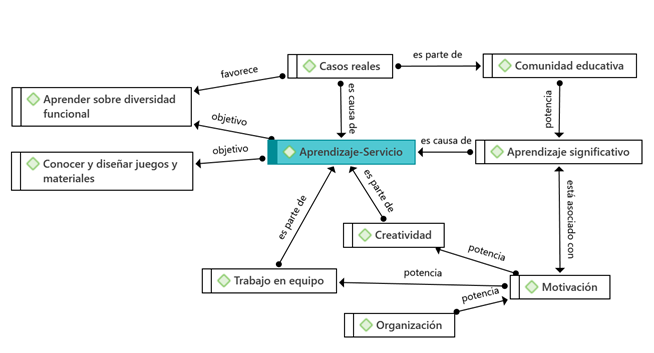
\includegraphics[width=0.8\textwidth]{figura 01.png}
\source{Elaboración propia.}
\end{figure}

En general, los estudiantes han valorado muy positivamente la posibilidad de trabajar con casos reales, ya que consideran que es una manera de conectar con su futuro profesional de forma eminentemente práctica. En esta misma línea, otro de los aspectos destacados por el alumnado ha sido la utilidad del aprendizaje. Mencionan que con su trabajo pueden ayudar a maestras y estudiantes a aprender con los juegos y materiales que han realizado. También se observa que estos casos pueden facilitar su comprensión y empatía hacia los niños con dificultades específicas de aprendizaje, ya que como menciona E7 “Saber que lo que hacemos de verdad llega a un niño, hace que te motive más. Mi equipo espera con ilusión que Pablo (nombre ficticio) disfrute con los juegos, y también nos ha hecho ver que en la discapacidad no todo es blanco o negro, hay cosas que se le darán mejor y otras peor, y nosotras tendremos que identificar sus dificultades para trabajar con ellos lo mejor posible”. Esta conexión entre los proyectos de ApS y las competencias profesionales adquiridas está ampliamente estudiado, por ejemplo, \textcite{jacoby_service-learning_2015} afirma que el Aprendizaje-Servicio es una forma de educación experiencial donde el aprendizaje ocurre a través de un ciclo de acción y reflexión a medida que los estudiantes buscan lograr objetivos reales para la comunidad.

Con respecto a la metodología en sí misma, se han sentido apoyados por sus compañeros en el trabajo cooperativo, así como por el profesorado a la hora de resolver dudas. Se ha observado que los estudiantes valoran el diseño de la propuesta pedagógica, destacando la importancia de implementar metodologías innovadoras que favorezcan su aprendizaje y les permitan desarrollar su creatividad, como ha sido el caso de este aprendizaje-servicio lúdico. El dinamismo del trabajo en grupo genera procesos de ayuda entre iguales y nuevos aprendizajes entre estudiantes con roles similares. Estos procesos favorecen las relaciones interpersonales entre los participantes, así como actitudes y aptitudes de colaboración \cite{claes_community_2021}.

También se menciona la importancia de crear sus propios recursos didácticos como actividad formativa dentro de la formación inicial del profesorado. E6 lo ejemplifica con la siguiente afirmación:  "me gustaban los juegos, pero no se me hubiera ocurrido que se pudieran aplicar así en la escuela. Me gustó que pudiéramos tratar de trabajar con ellos en las prácticas porque entonces puedo pensar en cómo usarlos con los niños y qué puedo trabajar con ellos". Es importante que a los estudiantes de formación inicial del profesorado se les enseñe a utilizar diferentes técnicas y herramientas para utilizar con sus futuros alumnos. Entre estos posibles recursos se encuentran los juegos por su valor educativo y social, ya que favorecen la construcción de relaciones interpersonales. \cite{turkoglu_effect_2019} y desarrollo intelectual y motor \cite{sala_video_2018,gumusdag_effects_2019}. Jugar es una parte importante del aprendizaje, además con el juego se satisfacen ciertas necesidades sociales, se promueve la imaginación, se facilita la asimilación de reglas y se favorece la construcción de afectividades y momentos de placer y diversión \cite{vygotskii_desarrollo_1982}; los juegos son recursos ampliamente estudiados por su eficacia en áreas de trabajo del desarrollo en niños y niñas con dificultades de aprendizaje \cite{kokkalia_role_2016,hanghoj_can_2018,jimenez_porta__impacto_2018,manzano-leon_testing_2021}.

Sin embargo, la propuesta metodológica puede presentar algunas desventajas. En primer lugar, requiere una gran implicación y formación del profesorado, y se deben disponer los recursos necesarios para la aplicación de la metodología. En segundo lugar, es necesario trabajar las habilidades sociales y cooperativas de los estudiantes universitarios, ya que si el alumnado no ha sido formado ni ha trabajado de manera cooperativa previamente, podría encontrarse con problemas técnicos y psicológicos a la hora de enfrentarse a este tipo de metodología. Aunque el discurso general del alumnado es muy positivo respecto al Aprendizaje-Servicio, al menos un grupo de estudiantes se dividió a mitad del semestre debido a problemas de comunicación entre sus miembros, por lo que la retroalimentación semanal entre el profesor y los equipos de estudiantes es fundamental para poder resolver los problemas que puedan surgir durante la práctica.

\section{Discusión y conclusiones}

Diseñar experiencias de aprendizaje activo y significativo para el alumnado es un gran reto en la educación universitaria. El objetivo de esta investigación ha sido analizar la percepción del alumnado del grado de Educación Infantil sobre la aplicación del Aprendizaje-Servicio lúdico. Para ello, se diseñó un ApS lúdico para las prácticas de la asignatura “Dificultades de Aprendizaje” donde el alumnado diseñó juegos y materiales para clases con estudiantes con diversidad funcional.

Estudios previos mencionan la importancia de enseñar contenidos prácticos a estudiantes universitarios y los beneficios del uso de casos reales y simulaciones \cite{kaufman_enhancing_2016,ferreira_simulacion_2021}, así como el carácter motivador del Aprendizaje-Servicio \cite{pu_improvement_2021,resch_using_2021}. Nuestros resultados confirmaron que el ApS lúdico en la formación inicial docente puede despertar la participación, la motivación, la sensibilización y el aprendizaje significativo del alumnado.

Tras los resultados de este Aprendizaje-Servicio, se pueden trazar algunas recomendaciones para futuras implementaciones en la educación universitaria. En primer lugar, que desde la primera sesión los alumnos puedan conocer el proyecto, el impacto social que puede lograr y cómo afecta a su sistema de evaluación de la asignatura, ya que esto puede favorecer el compromiso inicial. En segundo lugar, se recomienda que el profesor actúe como facilitador del aprendizaje y que esté disponible para poder ofrecer retroalimentación constante y ser reconocido su rol de guía a lo largo de la asignatura, con el objetivo de que pueda detectar posibles dificultades, problemas en los equipos de trabajo o pueda proponer mejoras en la continuación de los proyectos. Finalmente, para una mayor inmersión en los programas de ApS, se propone que el flujo de comunicación entre ambas partes (Estudiantes-Comunidad) pueda continuar durante todo el semestre académico para facilitar la sostenibilidad a largo plazo de estos proyectos.

Este estudio presenta limitaciones. En primer lugar, al no tratarse de una entrevista, no fue posible profundizar en las respuestas del alumnado participante que pudieran ofrecer una mayor perspectiva y reflexión sobre la metodología. En segundo lugar, al ser un estudio cualitativo y tener una muestra relativamente pequeña, los resultados no son generalizables. Futuras investigaciones podrían estudiar el impacto cuantitativo del ApS y la creación de materiales lúdicos en la formación inicial docente en las variables relacionadas con el rendimiento académico, la motivación y la adquisición de habilidades sociales a través de estudios experimentales longitudinales con un grupo control.

Se concluye que la experiencia del ApS lúdico ha sido positivamente evaluada por el alumnado. Principalmente debido a su valoración de casos prácticos reales, los cuales permiten llevar a la práctica los contenidos teóricos aprendidos, trabajando en herramientas didácticas que podrán utilizar con niños con dificultades de aprendizaje en su futuro profesional. La participación en la elaboración de juegos y materiales, a pesar del esfuerzo añadido para los equipos de estudiantes y el cuerpo docente, se percibe como una experiencia enriquecedora para el aprendizaje y sensibilización sobre la diversidad funcional, y especialmente motivadora debido a que ese esfuerzo tiene una utilidad real en la comunidad educativa.


\printbibliography\label{sec-bib}
% if the text is not in Portuguese, it might be necessary to use the code below instead to print the correct ABNT abbreviations [s.n.], [s.l.]
%\begin{portuguese}
%\printbibliography[title={Bibliography}]
%\end{portuguese}


%full list: conceptualization,datacuration,formalanalysis,funding,investigation,methodology,projadm,resources,software,supervision,validation,visualization,writing,review
\begin{contributors}[sec-contributors]
\authorcontribution{Ana Manzano-León}[conceptualization,methodology,software,formalanalysis,investigation,writing]
\authorcontribution{Ana María Ortiz-Colón}[validation,visualization,supervision]
\authorcontribution{Javier Rodríguez-Moreno}[validation,visualization,supervision]
\authorcontribution{José Manuel Aguilar-Parra}[conceptualization,methodology,validation,visualization,supervision]
\end{contributors}


\appendix 


\end{document}

